Supongamos que tienes un amigo daltónico que no puede distinguir entre una bola verde y una roja (no sabe si las bolas son de diferentes colores). Quieres probar que los colores de las bolas son diferentes pero tu amigo necesita algo más que tus palabras para estar convencido. ¿Hay alguna forma de probar que son de colores distintos sin revelar información sobre las bolas?

Una prueba de conocimiento cero (\emph{ZKP} o \emph{Zero-knowledge proof}) es una forma de probar la validez de una declaración sin revelar la declaración en sí. Un protocolo de conocimiento cero es un método mediante el cual una parte (el probador) puede demostrar a otra parte (el verificador) que algo es cierto, sin revelar ninguna información aparte del hecho de que la afirmación específica es cierta.

Un método ZKP para el problema inicial podría dividirse en los siguientes pasos:
\begin{enumerate}
     \item Tu amigo toma las bolas y te deja ver qué bola está en qué mano.
     
     \item Luego, decide si cambiar las bolas entre sus manos detrás de su espalda o mantenerlas en el orden original.
     
     \item A continuación, te presenta las bolas y te pregunta si las cambió o no. Como puedes distinguir la bola verde de la roja, puedes dar fácilmente la respuesta correcta.
     
     \item Tu amigo no está convencido, ya que tienes un 50 \% de posibilidades de adivinar correctamente si cambió las bolas o no y las bolas aún pueden ser del mismo color.
     
     \item Sin embargo, si se repite este experimento varias veces, eventualmente, la probabilidad de que adivines correctamente si cambió las bolas o no cada vez sería muy baja. Esto le permite a su amigo verificar que las bolas son de diferentes colores sin saber los colores reales de las bolas.
\end{enumerate}

\begin{figure}[ht]
    \centering
    \begin{subfigure}[c]{0.45\textwidth}
        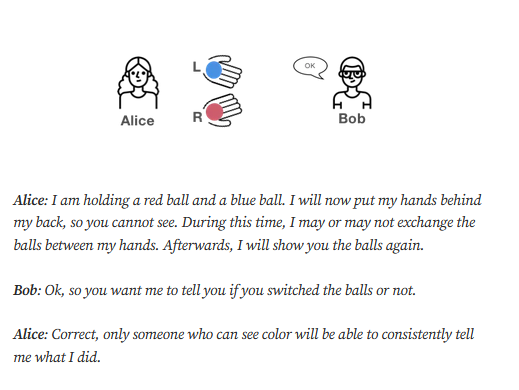
\includegraphics[width=\textwidth]{images/ballExample1.png}
    \end{subfigure}
    \begin{subfigure}[c]{0.45\textwidth}
        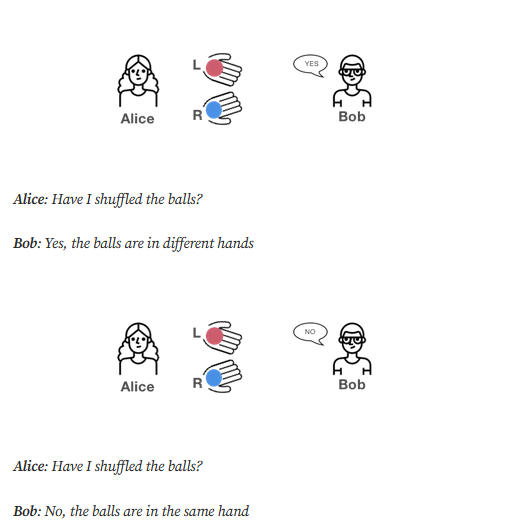
\includegraphics[width=\textwidth]{images/ballExample2.png}
    \end{subfigure}
    \caption{Ejemplo de prueba del color de las bolas \cite{Ball}}
    \label{im:ballExample}
\end{figure}
Las pruebas de conocimiento cero representaron un gran avance en la criptografía aplicada, permitiendo mejorar la seguridad de la información. Por ejemplo, podemos considerar como declaración ``Ser ciudadano de X país'', que querremos probar a un proveedor de servicios. Para probar esta declaración podemos utilizar ``pruebas'', como un pasaporte o un carnet de conducir. Pero hay problemas con este enfoque, principalmente la falta de privacidad. La información de identificación personal (\emph{Personal Identifiable Information}) compartida con servicios de terceros se almacena en bases de datos centrales, que en caso de que sufran algún ataque podría ser revelada a personas no deseadas. Dado que el robo de identidad se está convirtiendo en un problema crítico, como podemos ver en la figura \autoref{im:scams}, se piden más medios de protección de la privacidad para compartir información confidencial.

\begin{figure}[ht]
    \centering
    \begin{subfigure}[c]{0.9\textwidth}
        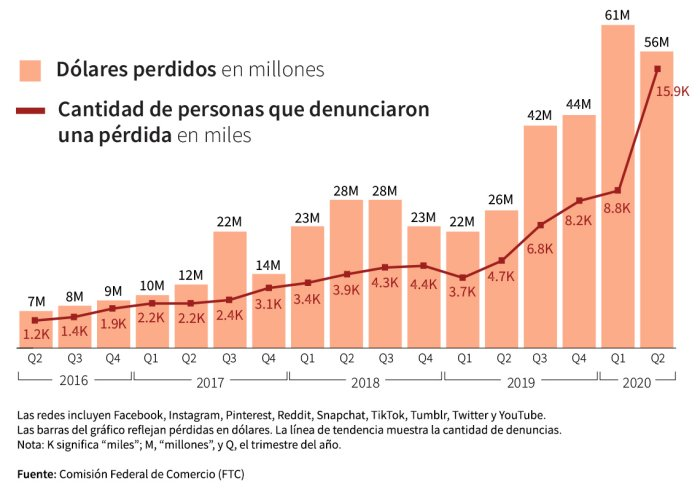
\includegraphics[width=\textwidth]{images/scams2.jpg}
    \end{subfigure}
    \caption{Pérdidas en redes sociales \cite{Fraudes}}
    \label{im:scams}
\end{figure}

Las pruebas de conocimiento cero resuelven este problema al eliminar la necesidad de revelar información para probar la validez de las afirmaciones. El protocolo de conocimiento cero utiliza la declaración (llamada ``testigo") como entrada para generar una prueba sucinta de su validez. Esta prueba proporciona fuertes garantías de que una declaración es verdadera sin exponer la información utilizada para crearla.

Volviendo a nuestro ejemplo anterior sobre la ciudadanía, la única evidencia que se necesita para probar la declaración de ciudadanía es una prueba de conocimiento cero. El verificador sólo tiene que verificar si ciertas propiedades de la prueba son verdaderas para estar convencido de que la declaración subyacente también lo es. Por ejemplo, más adelante veremos que podemos usar los protocolos de conocimiento cero para probar que un valor pertenece a un intervalo, sin dar ninguna información acerca de este valor. Esto nos permitiría probar que el número del pasaporte pertenece al intervalo correspondiente a un determinado país y así demostrar que es ciudadano de dicho país. O, si asociamos un número a cada país, podemos demostrar que el valor de su país pertenece a un intervalo que representa una región (como la Unión Europea) o a un continente sin revelar el país.

\section{Motivación}

Debido a la naturaleza de ZKP, puede utilizarse en muchos casos en los que la privacidad es deseable. Y lo que es más importante, también puede utilizarse como base para construir protocolos más sofisticados.

Gracias a la enorme capacidad de anonimato, privacidad y seguridad de este tipo de protocolos, sus principales casos de uso apuntan a sistema de comunicación seguro. Por ejemplo, los militares y las organizaciones de espionaje emplean este tipo de tecnología para asegurar comunicaciones. Esto con el fin de permitir el despliegue en campo de sistemas de comunicación muy seguros. También son muy utilizados en sistemas de autenticación, incluso vía web \cite{Motivacion}.

La tecnología además tiene amplios usos dentro de sistemas de votación seguros. Con las ZKP es posible que el votante pueda realizar su voto, demostrar que votó, pero de ninguna manera nadie podrá saber por qué opción ha votado. De esta forma, ZKP puede ayudar a los sistemas de votación a mantener el secreto del voto y otorgar transparencias a estos sistemas.

Otro caso de uso muy visto en la actualidad se da en las criptomonedas, como el caso de Zcash y Monero. Ambas criptomonedas implementan el uso de Zero Knowledge Protocol. Como es de esperar, la finalidad es poder garantizar la privacidad y anonimato de sus usuarios.

En el caso de Zcash, su sistema de pruebas zk-SNARKs está basado en el funcionamiento de ZKP. De estas, existe una evolución bajo el nombre zk-STARK que presentan mejores características en cuanto a seguridad y rendimiento, especialmente resistencia a computación cuántica. Por su lado, Monero y sus Bulletproof son también una adaptación de ZKP y Transacciones Confidenciales, lo que también le confiere un alto nivel de seguridad.

\begin{figure}[ht]
    \centering
    \begin{subfigure}[c]{0.45\textwidth}
        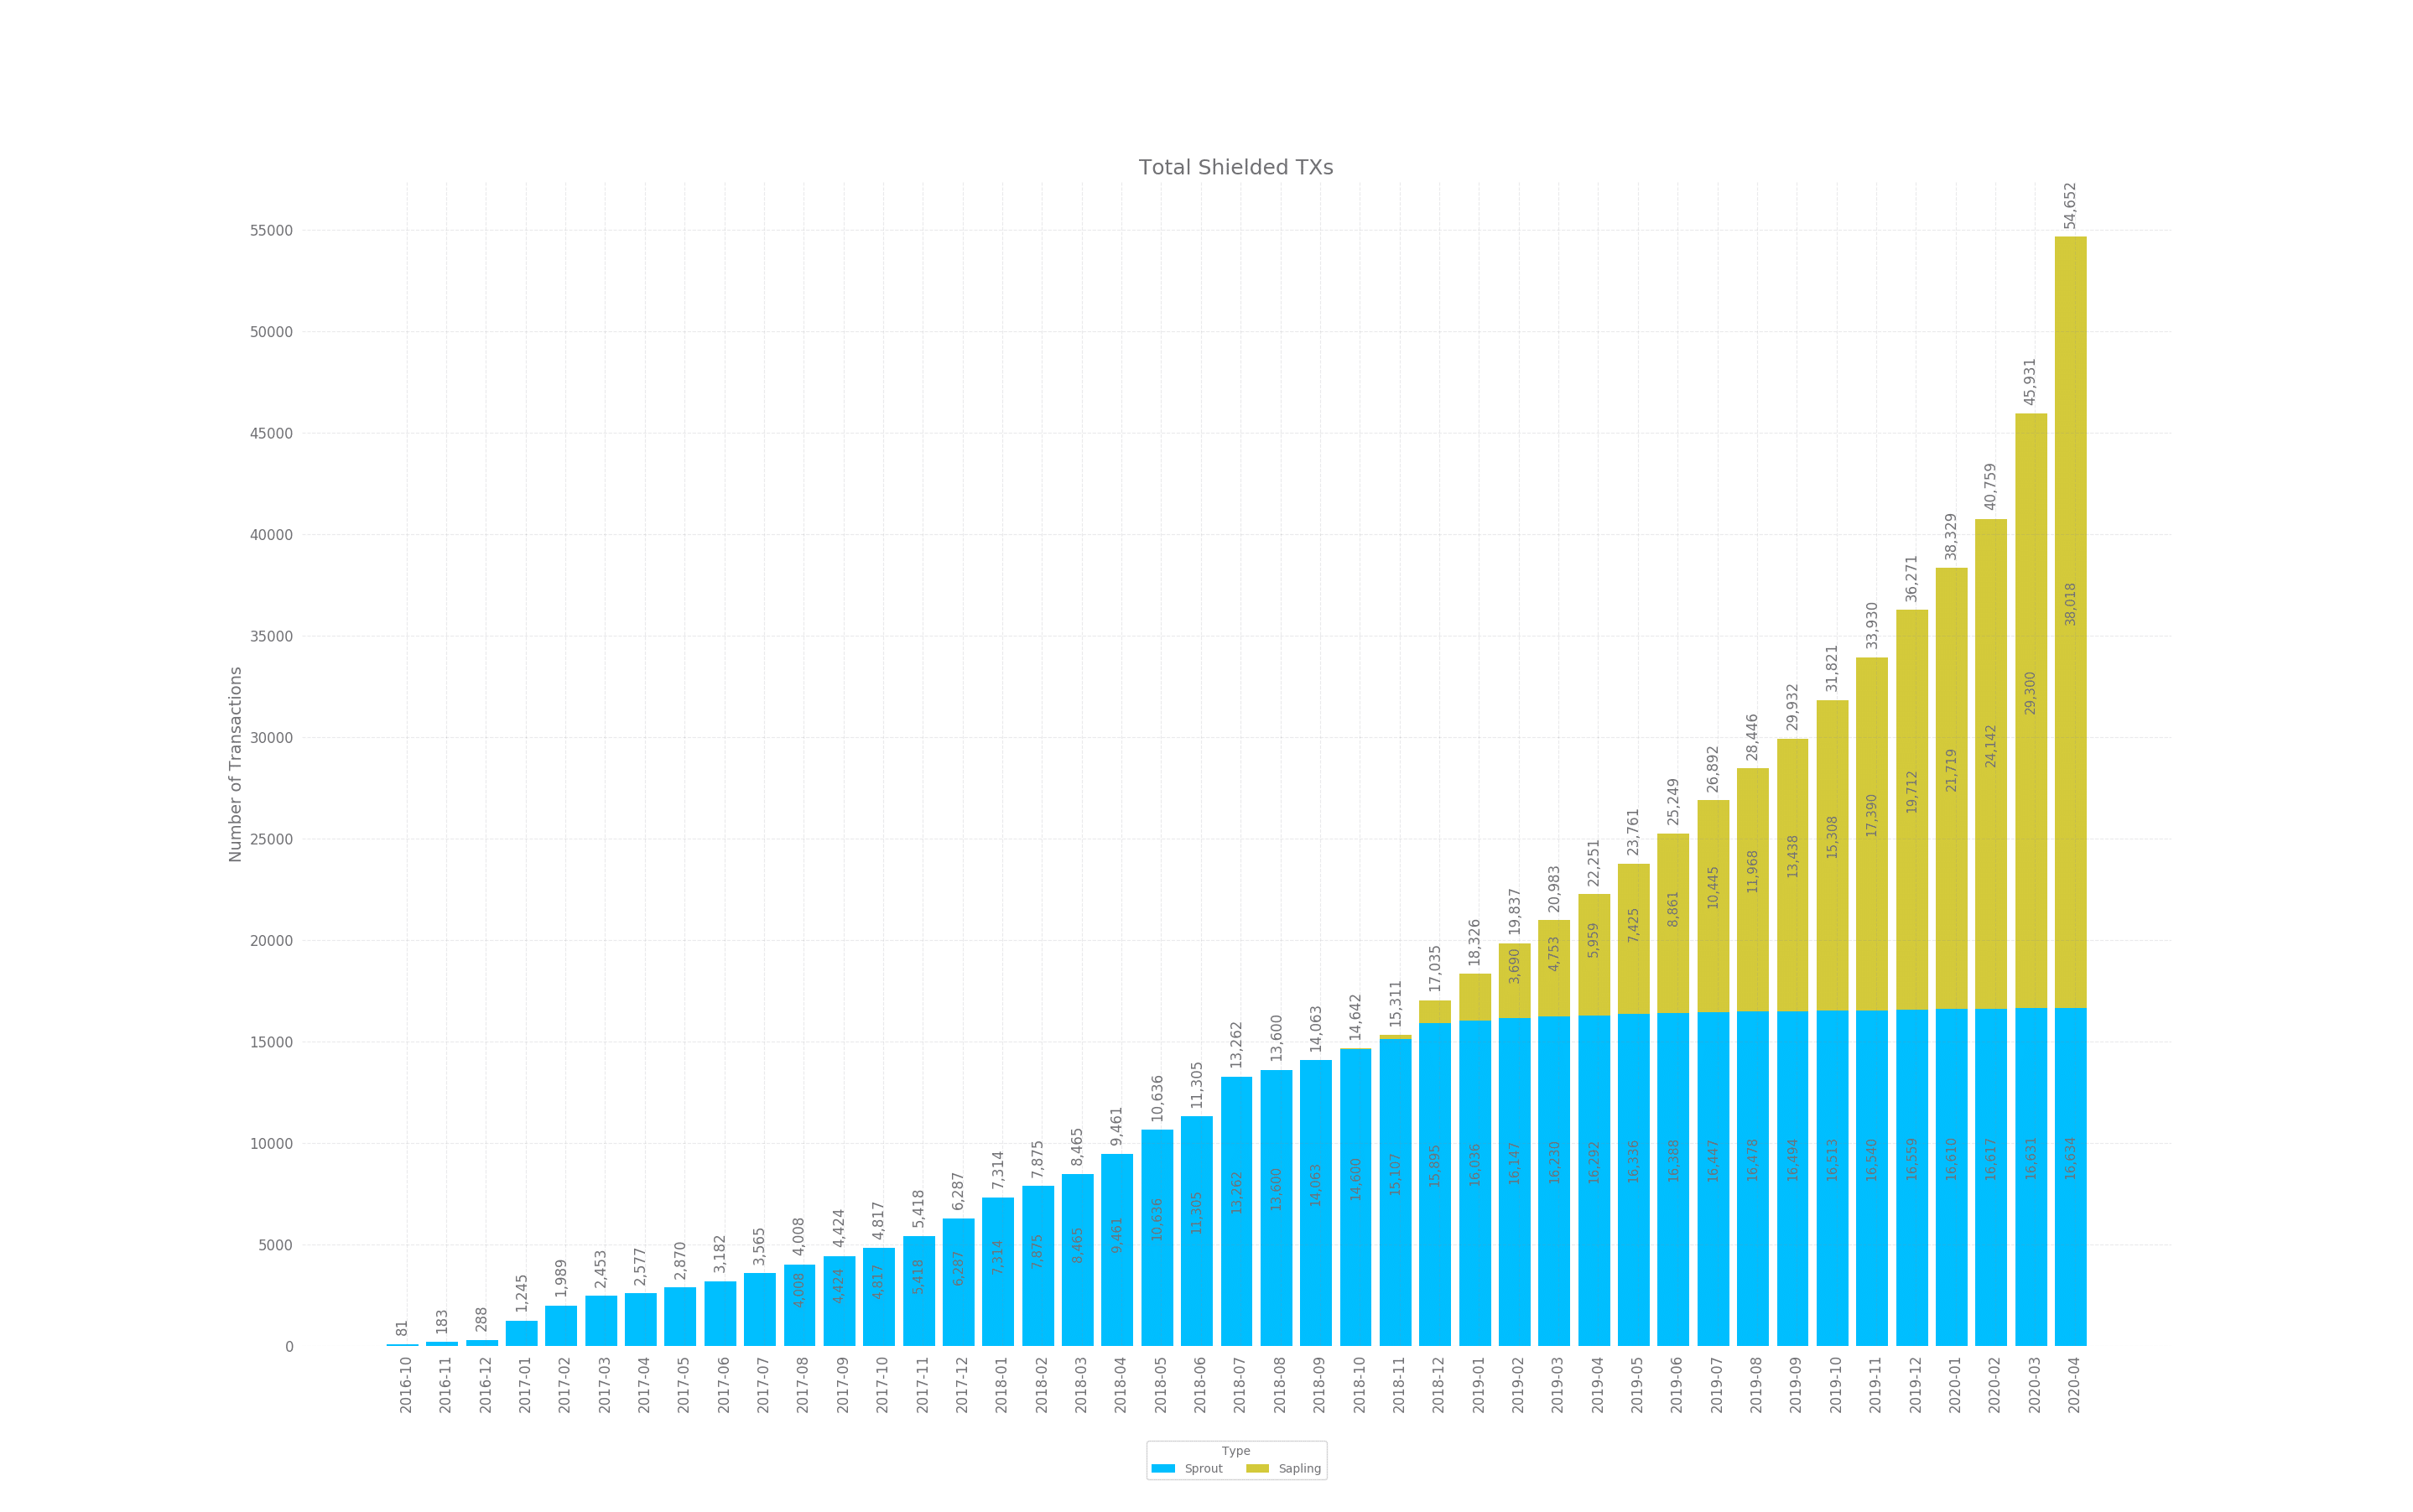
\includegraphics[width=\textwidth]{images/zcash.png}
        \caption{Aumento de usos de Zcash \cite{zCash}}
    \end{subfigure}
    \begin{subfigure}[c]{0.45\textwidth}
        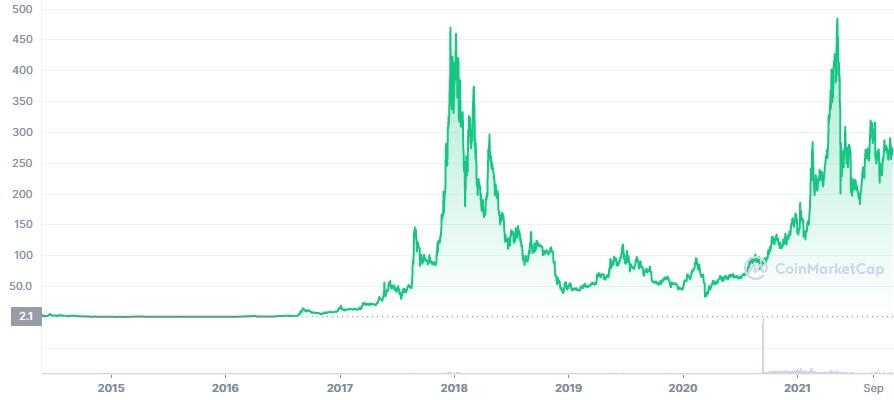
\includegraphics[width=\textwidth]{images/monero.jpg}
        \caption{Evolución del valor de Monero \cite{Monero}}
    \end{subfigure}
    
    \caption{Aumento de usos y valor de Zcash y Monero respectivamente}
    \label{im:motivacion}
\end{figure}

Como se puede ver en la \autoref{im:motivacion}, Zcash y  Monero han estado aumentando en valor y en uso en los últimos años, por lo que cabe esperar que los protocolos de conocimiento cero sean fundamentales en el próximo futuro y un aumento de la necesidad de profesionales en este ámbito. Además, como vimos en la \autoref{im:scams}, los robos de identidad y las pérdidas que estos conllevan es un tema importante en la actualidad, y los ZKP se pueden utilizar para aumentar la seguridad frente a estos robos permitiendo ocultar la información. Todo esto nos motiva en un estudio de estos protocolos.

Sin embargo, ya existen diversos artículos que definen estos protocolos y plantean nuevos algoritmos con diversas capacidades y ventajas. Por lo que, decidimos centrarnos en la docencia y, tal y como recomienda el artículo \emph{Transformation of the mathematics classroom with the internet} de 2020 \cite{Maths}, en lugar de crear un extenso documento acerca de su funcionamientos y de los distintos algoritmos relacionados (aunque si incluiremos un breve resumen para familiarizarse con su funcionamiento), decidimos crear una herramienta digital que permita interactuar con estos protocolos y así facilitar el aprendizaje sobre estas tecnologías.

\section{Solución Propuesta}

Para que pueda conocerse el funcionamiento de los protocolos de conocimiento cero, este trabajo intenta detallar un algoritmo de la forma más simple posible, implementando el algoritmo y ofreciendo al usuario una herramienta interactiva que le permite ver y modificar los valores, los distintos pasos y las salidas. De esta forma, siendo capaz de seguir paso a paso el algoritmo y modificando sus valores el usuario podrá comprender en mayor detalle el funcionamiento de un algoritmo de ZKP.

A continuación se detallan las contribuciones principales del presente trabajo fin de grado:
\begin{itemize}
    \item Explicación teórica de los protocolos de conocimientos cero, así como algunos posibles ejemplos de sus aplicaciones.
    
    \item Explicación y comparación entre distintos algoritmos de conocimiento cero. Además, se indica porqué decidimos centrarnos en uno de ellos en particular.

    \item Implementación del algoritmo seleccionado.

    \item Herramienta interactiva con la que se puede interactuar con dicho algoritmo, indicándole los valores que tomará como entrada y pudiendo modificar los resultados que se obtienen, para poder entender su funcionamiento.

    \item Comprobación del correcto funcionamiento del algoritmo implementado, realizando un número elevado de pruebas funcionales con distintos valores aleatorios.
\end{itemize}

\section{Estructura de la memoria}

Este trabajo se divide en los siguientes capítulos:
\begin{enumerate}[label=\textbf{{\arabic*.}}]
    \item \textbf{Introducción:} El objetivo de este capítulo es presentar un breve resumen de los protocolos de conocimiento cero que veremos en este trabajo, así como motivar su importancia y el porqué de este trabajo. Finalmente, se presenta un breve resumen de la estructura de la memoria y el contenido de cada capítulo.

    \item \textbf{Contexto de Zero Knowledge Proofs:} Esta sección sirve para motivar el estudio de los protocolos de conocimiento cero, demostrando su utilidad hoy en día con algunos ejemplos de posibles aplicaciones. Además, se estudian qué otras aportaciones hay en la implementación de los protocolos de conocimiento cero con fines docentes.

    \item \textbf{Marco teórico:} En esta sección se definen los protocolos de conocimiento cero, y se explica el funcionamiento de algunos en detalle. Además, se ofrecen ejemplos numéricos de uno de ellos, el que será el centro de este trabajo. Finalmente, se realiza una comparación entre los distintos algoritmos, justificando porque nos centramos en el algoritmo seleccionado.

    \item \textbf{Objetivos y Planificación:} Una vez que se comprende qué son los algoritmos de conocimiento cero y se hace una idea de cuál es su funcionamiento, se presentan los objetivos de este TFG. También se añade una planificación temporal con el objetivo de presentar el esfuerzo dedicado a cada una de las tareas y subtareas del presente trabajo.

    \item \textbf{Desarrollo de la propuesta:} En este capítulo se detalla la implementación que se ha realizado, tanto del algoritmo seleccionado como de la herramienta docente, con el objetivo de facilitar la comprensión de dicho algoritmo. Además, se explicarán las distintas herramientas utilizadas.

    \item \textbf{Conclusiones y líneas de trabajo futuro:} Finalmente, se ofrece un breve resumen de todo el trabajo y los resultados obtenidos, para analizar si este trabajo consigue completar los objetivos que planteados. También se indican las principales líneas de trabajo futuro que surgen tras la finalización del presente trabajo fin de grado.

    \item[·] \textbf{Anexos:} Su objetivo es servir como manual, para comprender como utilizar las distintas implementaciones de los algoritmos que se estudian en este trabajo, para que así se puedan utilizar y comprobar los resultados obtenidos con mayor facilidad.
\end{enumerate}
